
%%%%%%%%%%%%%%%%%%%%%%%%%%%%%%%%%%%%%%%%%%%%%%%%%%%%%%%%%%%%%%%%%%%%%%%%%%%%%%%%
%% ************************************************************************** %%
%% *                                Settings                                * %%
%% ************************************************************************** %%
%%%%%%%%%%%%%%%%%%%%%%%%%%%%%%%%%%%%%%%%%%%%%%%%%%%%%%%%%%%%%%%%%%%%%%%%%%%%%%%%
\documentclass{tron}

\loadglsentries{gls}
\glsaddall
\addbibresource{reference}
\usepackage{xcolor}  % Coloured text etc.
% fancy note style
% STYLE NOTES : v2.0
% additional fancy boxes
\usepackage[framemethod=TikZ]{mdframed}
%\usepackage{amsthm}

% gray color indicates [OPTIONAL READING]

%%%%%%%%%%%%%%%%%%%%%%%%%%%%%%
%Note
\newenvironment{note}[3][]{%
	\ifstrempty{#1}%
	{\mdfsetup{%
	frametitle={%
	\tikz[baseline=(current bounding box.east),outer sep=0pt]
	\node[anchor=east,rectangle,fill=#2]
	{\strut Note};}}
	}%
	{\mdfsetup{%
	frametitle={%
	\tikz[baseline=(current bounding box.east),outer sep=0pt]
	\node[anchor=east,rectangle,fill=#2]
	{\strut #1};}}%
	}%
	\mdfsetup{innertopmargin=0pt,skipabove=5pt,linecolor=#2,%
		linewidth=2pt,topline=true,%
		frametitleaboveskip=\dimexpr-\ht\strutbox\relax,
		backgroundcolor={white!90!#2}}
	\begin{mdframed}[]\relax%
	\label{#3}}{\end{mdframed}
}
\Crefname{note}{Note}{notes}

\newcommand{\createnoteenv}[6]{
	\refstepcounter{#6}%
	\ifstrempty{#1}%
	{\mdfsetup{%
	frametitle={%
	\tikz[baseline=(current bounding box.east),outer sep=0pt]
	\node[anchor=east,rectangle,fill=#3]
	{\strut #4~#5};}}
	}%
	{
		\mdfsetup{%
			frametitle={%
				\tikz[baseline=(current bounding box.east),outer sep=0pt]
				\node[anchor=east,rectangle,fill=#3]
				{\strut #4~#5:~#1};
			}
		}%
	}%
	\mdfsetup{innertopmargin=0pt,skipabove=5pt,linecolor=#3,%
	linewidth=2pt,topline=true,%
	frametitleaboveskip=\dimexpr-\ht\strutbox\relax,
	backgroundcolor={white!90!#3}}
	\begin{mdframed}[]\relax%
	\label{#2}
}

%%%%%%%%%%%%%%%%%%%%%%%%%%%%%%
%Definition
\newcounter{definition}[section] \setcounter{definition}{0}
\renewcommand{\thedefinition}{\arabic{section}.\arabic{definition}}
\newenvironment{definition}[2][]{%
	\createnoteenv{#1}{#2}{blue!40}{Definition}{\thedefinition}{definition}%
}{\end{mdframed}}
\newenvironment{definition*}[2][]{%
	\createnoteenv{#1}{#2}{gray!40}{Definition}{\thedefinition}{definition}%
}{\end{mdframed}}
\Crefname{definition}{Definition}{definitions}


%%%%%%%%%%%%%%%%%%%%%%%%%%%%%%
%theoremrem
\newcounter{theorem}[section] \setcounter{theorem}{0}
\renewcommand{\thetheorem}{\arabic{section}.\arabic{theorem}}
\newenvironment{theorem}[2][]{%
	\createnoteenv{#1}{#2}{cyan!40}{Theorem}{\thetheorem}{theorem}%
}{\end{mdframed}}
\newenvironment{theorem*}[2][]{%
	\createnoteenv{#1}{#2}{gray!40}{Theorem}{\thetheorem}{theorem}%
}{\end{mdframed}}
\Crefname{theorem}{Theorem}{theorems}

%%%%%%%%%%%%%%%%%%%%%%%%%%%%%%
%Proof
\newcounter{proof}[section]\setcounter{proof}{0}
\renewcommand{\theproof}{\arabic{section}.\arabic{proof}}
\newenvironment{proof}[2][]{%
	\createnoteenv{#1}{#2}{red!20}{Proof}{\theproof}{proof}%
}{\end{mdframed}}
\newenvironment{proof*}[2][]{%
	\createnoteenv{#1}{#2}{gray!40}{Proof}{\theproof}{proof}%
}{\end{mdframed}}
\Crefname{proof}{Proof}{proofs}


%%%%%%%%%%%%%%%%%%%%%%%%%%%%%%
%Alert
\newcounter{alert}[section]\setcounter{alert}{0}
\renewcommand{\thealert}{\arabic{section}.\arabic{alert}}
\newenvironment{alert}[2][]{%
	\createnoteenv{#1}{#2}{red!80}{Alert}{\thealert}{alert}%
}{\end{mdframed}}
\newenvironment{alert*}[2][]{%
	\createnoteenv{#1}{#2}{gray!40}{Alert}{\thealert}{alert}%
}{\end{mdframed}}
\Crefname{alert}{Alert}{alerts}

%%%%%%%%%%%%%%%%%%%%%%%%%%%%%%
%Answer
\newcounter{answer}[section]\setcounter{answer}{0}
\renewcommand{\theanswer}{\arabic{section}.\arabic{answer}}
\newenvironment{answer}[2][]{%
	\createnoteenv{#1}{#2}{orange!60}{Answer}{\theanswer}{answer}%
}{\end{mdframed}}
\newenvironment{answer*}[2][]{%
	\createnoteenv{#1}{#2}{gray!40}{Answer}{\theanswer}{answer}%
}{\end{mdframed}}
\Crefname{answer}{Answer}{answers}

%%%%%%%%%%%%%%%%%%%%%%%%%%%%%%
%Remark
\newcounter{remark}[section]\setcounter{remark}{0}
\renewcommand{\theremark}{\arabic{section}.\arabic{remark}}
\newenvironment{remark}[2][]{%
	\createnoteenv{#1}{#2}{orange!40}{Remark}{\theremark}{remark}%
}{\end{mdframed}}
\newenvironment{remark*}[2][]{%
	\createnoteenv{#1}{#2}{gray!40}{Remark}{\theremark}{remark}%
}{\end{mdframed}}
\Crefname{remark}{Remark}{remarks}


%%%%%%%%%%%%%%%%%%%%%%%%%%%%%%%
%%Example
%\newcounter{example}[section]\setcounter{example}{0}
%\renewcommand{\theexample}{\arabic{section}.\arabic{example}}
%\newenvironment{example}[2][]{%
%	\createnoteenv{#1}{#2}{blue!40!cyan!20}{Example}{\theexample}{example}%
%}{\end{mdframed}}
%\newenvironment{example*}[2][]{%
%	\createnoteenv{#1}{#2}{gray!40}{Example}{\theexample}{example}%
%}{\end{mdframed}}

%%%%%%%%%%%%%%%%%%%%%%%%%%%%%%
%Algorithm
\newcounter{algo}[section]\setcounter{algo}{0}
\renewcommand{\thealgo}{\arabic{algo}.\arabic{algo}}
\newenvironment{algo}[2][]{%
	\createnoteenv{#1}{#2}{yellow!90!brown!60}{Algorithm}{\thealgo}{algo}%
}{\end{mdframed}}
\newenvironment{algo*}[2][]{%
	\createnoteenv{#1}{#2}{gray!40}{Algorithm}{\thealgo}{algo}%
}{\end{mdframed}}
\Crefname{algo}{Algorithm}{algos}

%%%%%%%%%%%%%%%%%%%%%%%%%%%%%%
% CS480 - Exercise
%\setlength{\parskip}{1cm}
%\setlength{\parindent}{1cm}

%\tikzstyle{titregris} =
%[draw=gray,fill=white, shading = exersicetitle, %
%text=gray, rectangle, rounded corners, right,minimum height=.3cm]
%\pgfdeclarehorizontalshading{exersicebackground}{100bp}
%{color(0bp)=(green!40); color(100bp)=(black!5)}
%\pgfdeclarehorizontalshading{exersicetitle}{100bp}
%{color(0bp)=(red!40);color(100bp)=(black!5)}
%\newcounter{exercise}
%\renewcommand*\theexercise{exercice \textbf{Exercice}~n\arabic{exercise}}
%\makeatletter
%\def\mdf@@exercisepoints{}%new mdframed key:
%\define@key{mdf}{exercisepoints}{%
%\def\mdf@@exercisepoints{#1}
%}
%
%\mdfdefinestyle{theoremstyle}{%
%outerlinewidth=0.01em,linecolor=black,middlelinewidth=0.5pt,%
%frametitlerule=true,roundcorner=2pt,%
%apptotikzsetting={\tikzset{mfframetitlebackground/.append style={%
%shade,left color=white, right color=blue!20}}},
%frametitlerulecolor=black,innertopmargin=1\baselineskip,%green!60,
%innerbottommargin=0.5\baselineskip,
%frametitlerulewidth=0.1pt,
%innertopmargin=0.7\topskip,skipabove={\dimexpr0.2\baselineskip+0.1\topskip\relax},
%frametitleaboveskip=1pt,
%frametitlebelowskip=1pt
%}
%\mdtheorem[style=theoremstyle]{exercise}{\textbf{Exercise}}

\newcounter{exercise}[section]\setcounter{exercise}{0}
\renewcommand{\theexercise}{\arabic{exercise}}
\newenvironment{exercise}[2][]{%
	\createnoteenv{#1}{#2}{gray!40}{Exercise}{\theexercise}{exercise}%
}{\end{mdframed}}
\newenvironment{exercise*}[2][]{%
	\createnoteenv{#1}{#2}{gray!40}{Exercise}{\theexercise}{exercise}%
}{\end{mdframed}}

\Crefname{exercise}{Exercise}{exercises}


%%%%%%%%%%%%%%%%%%%%%%%%%%%%%%
%Examples
% {

%     \section{Theorem and lemma examples with title}
%     \begin{theorem}[Pythagoras' theorem]{theorem:pythagoras}
%     In a right triangle, the square of the hypotenuse is equal to the sum of the squares of the catheti.
%     \[a^2+b^2=c^2\]
%     \end{theorem}
%     In mathematics, the Pythagorean theorem, also known as Pythagoras' theorem (see theorem \ref{theorem:pythagoras}), is a relation in Euclidean geometry among the three sides of a right triangle.
%     
%     \begin{definition}[B\'ezout's identity]{def:bezout}
%     Let $a$ and $b$ be nonzero integers and let $d$ be their greatest common divisor. Then there exist integers $x$ and $y$ such that:
%     \[ax+by=d\]
%     \end{definition}
%     This is a reference to Bezout's lemma \ref{def:bezout}
%     
%     
%     \section{Theorem and proof examples without title}
%     
%     \begin{theorem}[]{theorem:theorem1}
%     There exist two irrational numbers $x$, $y$ such that $x^y$ is rational.
%     \end{theorem}
%     
%     \begin{proof}[]{proof:proof1}
%     If $x=y=\sqrt{2}$ is an example, then we are done; otherwise $\sqrt{2}^{\sqrt{2}}$ is irrational, in which case taking $x=\sqrt{2}^{\sqrt{2}}$ and $y=\sqrt{2}$ gives us:
%     \[\bigg(\sqrt{2}^{\sqrt{2}}\bigg)^{\sqrt{2}}=\sqrt{2}^{\sqrt{2}\sqrt{2}}=\sqrt{2}^{2}=2.\]
%     \end{proof}
%
%     \begin{alert}[]{alert:alert1}
%     If $x=y=\sqrt{2}$ is an example, then we are done; otherwise $\sqrt{2}^{\sqrt{2}}$ is irrational, in which case taking $x=\sqrt{2}^{\sqrt{2}}$ and $y=\sqrt{2}$ gives us:
%     \[\bigg(\sqrt{2}^{\sqrt{2}}\bigg)^{\sqrt{2}}=\sqrt{2}^{\sqrt{2}\sqrt{2}}=\sqrt{2}^{2}=2.\]
%     \end{alert}
%     
%     \begin{remark}[]{alert:alert1}
%     If $x=y=\sqrt{2}$ is an example, then we are done; otherwise $\sqrt{2}^{\sqrt{2}}$ is irrational, in which case taking $x=\sqrt{2}^{\sqrt{2}}$ and $y=\sqrt{2}$ gives us:
%     \[\bigg(\sqrt{2}^{\sqrt{2}}\bigg)^{\sqrt{2}}=\sqrt{2}^{\sqrt{2}\sqrt{2}}=\sqrt{2}^{2}=2.\]
%     \end{remark}
%     
%     
%          \begin{exercise}[]{alert:alert1}
%     If $x=y=\sqrt{2}$ is an example, then we are done; otherwise $\sqrt{2}^{\sqrt{2}}$ is irrational, in which case taking $x=\sqrt{2}^{\sqrt{2}}$ and $y=\sqrt{2}$ gives us:
%     \[\bigg(\sqrt{2}^{\sqrt{2}}\bigg)^{\sqrt{2}}=\sqrt{2}^{\sqrt{2}\sqrt{2}}=\sqrt{2}^{2}=2.\]
%     \end{exercise}
%     
%     \begin{algo}[]{algorithm:alert1}
%     If $x=y=\sqrt{2}$ is an example, then we are done; otherwise $\sqrt{2}^{\sqrt{2}}$ is irrational, in which case taking $x=\sqrt{2}^{\sqrt{2}}$ and $y=\sqrt{2}$ gives us:
%     \[\bigg(\sqrt{2}^{\sqrt{2}}\bigg)^{\sqrt{2}}=\sqrt{2}^{\sqrt{2}\sqrt{2}}=\sqrt{2}^{2}=2.\]
%     \end{algo}
%     
%     \begin{note}[Goal]{pink}{note:goal}
%     If $x=y=\sqrt{2}$ is an example, then we are done; otherwise $\sqrt{2}^{\sqrt{2}}$ is irrational, in which case taking $x=\sqrt{2}^{\sqrt{2}}$ and $y=\sqrt{2}$ gives us:
%     \[\bigg(\sqrt{2}^{\sqrt{2}}\bigg)^{\sqrt{2}}=\sqrt{2}^{\sqrt{2}\sqrt{2}}=\sqrt{2}^{2}=2.\]
%     \end{note}

% }
%\usepackage{lipsum}                     % Dummytext
\usepackage{xargs}                      % Use more than one optional parameter in a new commands
\usepackage[colorinlistoftodos,prependcaption,textsize=normalsize]{todonotes}
%
\newcommandx{\unsure}[2][1=]{\todo[linecolor=red,backgroundcolor=red!25,bordercolor=red,#1]{#2}}
\newcommandx{\change}[2][1=]{\todo[linecolor=blue,backgroundcolor=blue!25,bordercolor=blue,#1]{#2}}
\newcommandx{\info}[2][1=]{\todo[linecolor=OliveGreen,backgroundcolor=OliveGreen!25,bordercolor=OliveGreen,#1]{#2}}
\newcommandx{\improvement}[2][1=]{\todo[linecolor=Plum,backgroundcolor=Plum!25,bordercolor=Plum,#1]{#2}}
\newcommandx{\thiswillnotshow}[2][1=]{\todo[disable,#1]{#2}}
%
\preto\printlistoftodos{
    \listoftodos[Todo List]
}

% EXAMPLES:
    % \todo[inline]{The original todo note withouth changed colours.\newline Here's another line.}
    % \lipsum[11]\unsure{Is this correct?}\unsure{I'm unsure about also!}
    % \lipsum[11]\change{Change this!}
    % \lipsum[11]\info{This can help me in chapter seven!}
    % \lipsum[11]\improvement{This really needs to be improved!\newline\newline What was I thinking?!}
    % \lipsum[11]
    % \thiswillnotshow{This is hidden since option `disable' is chosen!}
    % \improvement[inline]{The following section needs to be rewritten!}
    % \lipsum[11]
    % \newpage
    % \listoftodos[Notes]
%%%  Equation Condition
\newenvironment{eqconditions}
  {\par\vspace{\abovedisplayskip}\noindent\begin{tabular}{>{$}l<{$} @{${}={}$} l}}
  {\end{tabular}\par\vspace{\belowdisplayskip}}
\newenvironment{eqconditions*}
  {\noindent\begin{tabular}{>{$}l<{$} @{${}={}$} l}}
  {\end{tabular}}
%%% introduce 4th depth with \paragraph command
\usepackage{titlesec}
\setcounter{secnumdepth}{4}
\titleformat{\paragraph}
{\normalfont\normalsize\bfseries}{\theparagraph}{1em}{}
\titlespacing*{\paragraph}
{0pt}{3.25ex plus 1ex minus .2ex}{1.5ex plus .2ex}

%%% enumeration reference
% constraint
\newlist{constraint-list}{enumerate}{1}
\setlist[constraint-list,1]{leftmargin=*, label= \Roman*}
\creflabelformat{Constraint}{#2#1#3}
\crefname{constraint-listi}{Constraint}{position}
% criteria
\newlist{criteria-list}{enumerate}{1}
\setlist[criteria-list,1]{leftmargin=*, label= \Roman*}
\creflabelformat{Criterion}{#2#1#3}
\crefname{criteria-listi}{Criterion}{position}
% property
\newlist{property-list}{enumerate}{1}
\setlist[property-list,1]{leftmargin=*, label= \Roman*}
\creflabelformat{Property}{#2#1#3}
\crefname{property-listi}{Property}{position}
% assumption
\newlist{assumption-list}{enumerate}{1}
\setlist[assumption-list,1]{leftmargin=*, label= \Roman*}
\creflabelformat{Assumption}{#2#1#3}
\crefname{assumption-listi}{Assumption}{position}

% custom math command
\newcommand{\unit}[1]{\left[\si{#1}\right]}

% additional math packages
\usepackage{physics}
\usepackage{cancel}

% TODO Flags
\newcommand\TODO[1]{{\textcolor{red}{\textbf{#1}}}}
\newcommand\COMMENT[1]{\hl{#1}}

% Custom Format
% \usepackage{float}
% \usepackage[table]{xcolor}
% \usepackage{soul}
\usepackage{multirow}
\usepackage{caption} 
\captionsetup[table]{skip=3pt}
\captionsetup[figure]{skip=0pt}
\titlespacing*{\section}
{0pt}{10pt}{3pt}
\titlespacing*{\subsection}
{0pt}{8pt}{3pt}
\titlespacing*{\subsubsection}
{0pt}{8pt}{3pt}
%hide the highlight box
\hypersetup{
    colorlinks,
    linkcolor={black!50!black},
    citecolor={black!50!blue},
    urlcolor={black!80!black}
}%hide the highlight box

% table formatting
% \setlength{\arrayrulewidth}{1mm}
% \setlength{\tabcolsep}{18pt}
% \renewcommand{\arraystretch}{2.5}
\usepackage{array}
\newcolumntype{C}[1]{>{\centering\let\newline\\\arraybackslash\hspace{0pt}}m{#1}}

% custom math symbol
%% CS 480 %%
\newcommand{\bm}[1]{\mathbf{#1}}
%%%%%%%%%%%%
\newcommand{\RR}{\mathds{R}}
\newcommand{\Id}{\mathbb{I}}
\newcommand{\NN}{\mathds{N}}
\newcommand{\sign}{\mathop{\mathrm{sign}}}
\newcommand{\diag}{\mathop{\mathrm{diag}}}
\newcommand{\argmin}{\mathop{\mathrm{argmin}}}
\newcommand{\zero}{\mathbf{0}}
\newcommand{\one}{\mathbf{1}}
\newcommand{\av}{\mathbf{a}}
\newcommand{\bv}{\mathbf{b}}
\newcommand{\sv}{\mathbf{s}}
\newcommand{\Xv}{\mathbf{X}}
\newcommand{\Yv}{\mathbf{Y}}
\newcommand{\wv}{\mathbf{w}}
\newcommand{\xv}{\mathbf{x}}
\newcommand{\yv}{\mathbf{y}}
\newcommand{\zv}{\mathbf{z}}
\newcommand{\uv}{\mathbf{u}}
\newcommand{\rv}{\mathbf{r}}
\newcommand{\inner}[2]{\langle #1, #2 \rangle}
\newcommand{\red}[1]{{\color{red}#1}}
\newcommand{\blue}[1]{{\color{blue}#1}}
\newcommand{\magenta}[1]{{\color{magenta}#1}}


\newcommand{\ea}{{et al.}\xspace}
\newcommand{\eg}{{e.g.}\xspace}
\newcommand{\ie}{{i.e.}\xspace}
\newcommand{\iid}{{i.i.d.}\xspace}
\newcommand{\cf}{{cf.}\xspace}
\newcommand{\wrt}{{w.r.t.}\xspace}
\newcommand{\aka}{{a.k.a.}\xspace}
\newcommand{\etc}{{etc.}\xspace}
\newcommand{\sgm}{\mathsf{sgm}}
\newcommand{\Dc}{\mathcal{D}}
\newcommand{\ans}[1]{{\textcolor{orange}{\textsf{Ans}: #1}}}



% extra mod
\newcommand{\mref}[1]{\underline{\textbf{\hypersetup{linkcolor=orange}\Cref{#1}\hypersetup{linkcolor=blue}}}}

%%%%%%%%%%%%%%%%%%%%%%%%%%%%%%%%%%%%%%%%%%%%%%%%%%%%%%%%%%%%%%%%%%%%%%%%%%%%%%%%
% Make sure the following block contains the correct information               %
%%%%%%%%%%%%%%%%%%%%%%%%%%%%%%%%%%%%%%%%%%%%%%%%%%%%%%%%%%%%%%%%%%%%%%%%%%%%%%%%
\reporttitle{CS 480 - Homework 1}
% \selfstudy % comment this line if this is not a self study report 
% \employername{Employer Name}
% \employerstreetaddress{Employer Address}
% \employerlocation{City, Provice, Country}
\university{University of Waterloo}
\faculty{Cheriton School of Computer Science}%Faculty of Engineering
\department{}%Department of Systems Design Engineering
\groupnumber{1}
\authornameA{Jianxiang (Jack) Xu}
\studentnumberA{20658861}
\reportdate{\today}
%\confidential{1} % comment this line if this is not a confidential report
%\authorstreetaddress{##}
%\authorlocation{##}
%\authorpostalcode{##}
\useheader % comment this line if no need for header
%%%%%%%%%%%%%%%%%%%%%%%%%%%%%%%%%%%%%%%%%%%%%%%%%%%%%%%%%%%%%%%%%%%%%%%%%%%%%%%%
% end of information block...                                                  %
%%%%%%%%%%%%%%%%%%%%%%%%%%%%%%%%%%%%%%%%%%%%%%%%%%%%%%%%%%%%%%%%%%%%%%%%%%%%%%%%

\begin{document}
%%%%%%%%%%%%%%%%%%%%%%%%%%%%%%%%%%%%%%%%%%%%%%%%%%%%%%%%%%%%%%%%%%%%%%%%%%%%%%%%
%% ************************************************************************** %%
%% *                               Title Page                               * %%
%% ************************************************************************** %%
%%%%%%%%%%%%%%%%%%%%%%%%%%%%%%%%%%%%%%%%%%%%%%%%%%%%%%%%%%%%%%%%%%%%%%%%%%%%%%%%
\maketitle
%%%%%%%%%%%%%%%%%%%%%%%%%%%%%%%%%%%%%%%%%%%%%%%%%%%%%%%%%%%%%%%%%%%%%%%%%%%%%%%%
%% ************************************************************************** %%
%% *                           Table of Contents                            * %%
%% ************************************************************************** %%
%%%%%%%%%%%%%%%%%%%%%%%%%%%%%%%%%%%%%%%%%%%%%%%%%%%%%%%%%%%%%%%%%%%%%%%%%%%%%%%%
% \tableofcontents
%%%%%%%%%%%%%%%%%%%%%%%%%%%%%%%%%%%%%%%%%%%%%%%%%%%%%%%%%%%%%%%%%%%%%%%%%%%%%%%%
%% ************************************************************************** %%
%% *                            List of Figures                             * %%
%% ************************************************************************** %%
%%%%%%%%%%%%%%%%%%%%%%%%%%%%%%%%%%%%%%%%%%%%%%%%%%%%%%%%%%%%%%%%%%%%%%%%%%%%%%%%
% \listoffigures
%%%%%%%%%%%%%%%%%%%%%%%%%%%%%%%%%%%%%%%%%%%%%%%%%%%%%%%%%%%%%%%%%%%%%%%%%%%%%%%%
%% ************************************************************************** %%
%% *                             List of Tables                             * %%
%% ************************************************************************** %%
%%%%%%%%%%%%%%%%%%%%%%%%%%%%%%%%%%%%%%%%%%%%%%%%%%%%%%%%%%%%%%%%%%%%%%%%%%%%%%%%
% \listoftables
%%%%%%%%%%%%%%%%%%%%%%%%%%%%%%%%%%%%%%%%%%%%%%%%%%%%%%%%%%%%%%%%%%%%%%%%%%%%%%%%
%% ************************************************************************** %%
%% *                              MAIN BODY                                 * %%
%% ************************************************************************** %%
%%%%%%%%%%%%%%%%%%%%%%%%%%%%%%%%%%%%%%%%%%%%%%%%%%%%%%%%%%%%%%
\clearpage
\pagenumbering{arabic}
\setcounter{page}{1}
\setlength{\parskip}{5pt}
\newpage

%%%%%%%%%%%%%%%%%%%%%%%%%%%%%%%%%%%
%%%%% Intro.  %%%%%%
%%%%%%%%%%%%%%%%%%%%%%%%%%%%%%%%%%%
\begin{center}
  \large{\textbf{CS480/680: Introduction to Machine Learning} \\ Homework 2\\ \red{Due: 11:59 pm, February 12, 2021}}
\end{center}


%%%%%%%%%%%%%%%%
%%%%% Ex 1 %%%%%
%%%%%%%%%%%%%%%%
\setcounter{section}{1}
\begin{exercise}[$k$-Nearest Neighbours (5 pts)]{}
The KNN-dataset provides a 4x4 representation of the handwritten digits 5, 6, and 8. Using the notebook provided, train a KNN classifier using 5-fold cross validation to determine the optimal k-value for this task.

\begin{enumerate}
\item (3 pt) Create a graph that shows the average accuracy based on 5-fold cross validation when varying the number of neighbours from 1 to 30.

\ans{\mref{ans:1:1}}

\item (1 pt) Report the best hyperparameter found by 5-fold cross-validation and the cross-validation accuracy.

\ans{\mref{ans:1:2}} 

\item (1 pt) Report the test accuracy based on the best hyperparameter.

\ans{\mref{ans:1:3}} 
\end{enumerate}
\end{exercise}


% --- ANS --- %
\begin{answer}[KNN classifier with 5-fold cross validation]{ans:1:1}
	{	
			\centering
			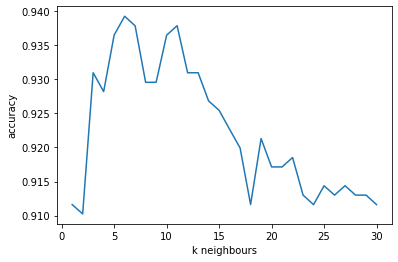
\includegraphics[height=200px]{Fig/q1}
	      	\captionof{figure}{KNN Accuracy vs. K-size  \label{fig:q1:1:knn}}
	}	
	\textbf{See code in the jupyter submission.}
\end{answer}

% --- ANS --- %
\begin{answer}[Best Hyperparameter]{ans:1:2}
	From the output below, we may find the best hyperparamter is $k=5$, with 93.92\% cross-validation accuracy and 92.31\% test accuracy.
	
	\begin{lstlisting}[language=python, style=mystyle:output]
		best # of neighbours k: 5
		best cross validation accuracy: 0.9392432950191572
		test accuracy: 0.9230769230769231
	\end{lstlisting}
	\vspace{-20pt}
\end{answer}

% --- ANS --- %
\begin{answer}[Test Accuracy]{ans:1:3}
	As reported in \mref{ans:1:2}, the final test accuracy is 92.31\%.
\end{answer}



%%%%%%%%%%%%%%%
%%%% Ex 2 %%%%%
%%%%%%%%%%%%%%%
\newpage
\setcounter{section}{2}
\begin{exercise}[Poisson Regression (4 pts)]{}
Recall that in logistic regression we assumed the \emph{binary} label $Y_i \in \{0,1\}$ follows the Bernoulli distribution: $\Pr(Y_i = 1 | X_i) = p_i$, where $p_i$ also happens to be the mean. Under the independence assumption we derived the log-likelihood function:
\begin{align}
\sum_{i=1}^n (1-y_i) \log(1-p_i) + y_i \log(p_i).
\end{align}
Then, we parameterized the mean parameter $p_i$ through the logit transform:
\begin{align}
\log\frac{p_i}{1-p_i} = \wv^\top \xv_i + b, \quad \mbox{ or equivalently } \quad p_i = \frac{1}{1+\exp(-\wv^\top \xv_i - b)}.
\end{align}
Lastly, we found the weight vector $\wv$ and $b$ by maximizing the log-likelihood function. 

In the following we generalize the above idea to the case where $Y_i \in \mathds{N}$, i.e., $Y_i$ can take any natural number (for instance, when we are interested in predicting the number of customers or network packages).

\begin{enumerate}
\item (1 pt) Naturally, we assume $Y_i \in \mathds{N}$ follows the Poisson distribution (with mean $\mu_i > 0$):
	\begin{align}
	\Pr(Y_i = k | X_i) = \frac{\mu_i^k}{k!} \exp(-\mu_i), ~~ k = 0, 1, 2, \ldots. \label{eqn:poisson-pdf}
	\end{align}
	Given a dataset $\Dc = \{\xv_i, y_i\}_{i=1}^n$, what is the log-likelihood function (of $\mu_i$'s) given $\Dc$?

\ans{\mref{ans:2:1}} 
	
\item (1 pt) Can you give some justification of the parameterization below?
	\begin{align}
	\log\mu_i = \wv^\top \xv_i + b. \label{eqn:log-param}
	\end{align}

\ans{\mref{ans:2:2}} 
	
\item (1 pt) Based on the above, write down the objective function for Poisson regression. Please specify the optimization variables and whether you are maximizing or minimizing. [Constants can be dropped.]

\ans{\mref{ans:2:3}} 
	
\item (1 pt) Compute the gradient of your objective function above and formulate a gradient algorithm for finding the weight vector $\wv$ and $b$. 
	
\ans{\mref{ans:2:4}} 

\end{enumerate}
\end{exercise}


% --- ANS --- %

%https://web.stanford.edu/class/archive/stats/stats200/stats200.1172/Lecture27.pdf
%https://www.cs.princeton.edu/~bee/courses/lec/lec_jan29.pdf
%https://towardsdatascience.com/generalized-linear-models-8738ae0fb97d
\newpage
\setcounter{answer}{0}
\begin{answer}[Log-likelihood Function]{ans:2:1}
	Since $Y_i={y_i} \in \mathds{N}$ are \iid Poisson random variables, we may obtain the likelihood function ($L(\mu_i)$):
	\begin{align}
		L(\mu_i) 	& = \Pr \left( Y_1=y_1, \dots, Y_n=y_n | X_1=x_1, \dots X_n=x_n \right) \\
					& = \prod_{i=1}^n {\Pr (Y_i = y_i | X_i)} \\
					& = \prod_{i=1}^n { \frac{\mu_i^{y_i}}{{y_i}!} \exp(-\mu_i) } 
	\end{align}
	
	Since maximizing the likelihood function is equivalent to maximizing its log function, hence we may take log of the entire likelihood function $L(\mu_i)$ from above to compute the log-likelihood:
	
	\begin{align}
		l(\mu_i) 	& = \log(L(\mu_i)) = \log \left( \prod_{i=1}^n { \frac{\mu_i^{y_i}}{{y_i}!} \exp(-\mu_i) } \right) \\
					& = \sum_{i=1}^n \left(  \log(\exp(-\mu_i)) + \log(\mu_i^{y_i}) - \log({y_i}!) \right) \\
					& = \sum_{i=1}^n \left(  -\mu_i + {y_i}\log(\mu_i) - \log({y_i}!) \right) 
	\end{align}
\end{answer}

\newpage
\begin{answer}[Justification of the parameterization]{ans:2:2}
	The goal in linear regression is to find some best fit factor $\wv$ and bias $b$ that will allow us to map $\xv_i$ to some model $y$. Similarly, we transfer the space into a distribution model, where the output $y_i$ is sampled from a normal distribution (Poisson distribution in this case). 
	
	Hence, 
	\begin{align}
		y \sim \mathcal{N}(y; \mu, \sigma^2), \quad \text{where } \mu_i &= \wv^\top \xv_i + b.
	\end{align}
	
	However, in our case, the distribution is Poisson and $\mu_i > 0$. Since $\wv^\top \xv_i + b$ has to be mapped to $(-\infty, \infty)$, $log(\mu_i)$ is a reasonable mapping strategy to transfer $\mu_i > 0$ to $(-\infty, \infty)$. 
	
	Hence,
	\begin{align}
		y \sim Po(y; \mu, \sigma^2), \quad \text{where } \log(\mu_i) &= \wv^\top \xv_i + b.
	\end{align}

\end{answer}

\newpage
\begin{answer}[Objective Function for Poisson Regression]{ans:2:3}
	From \Cref{eqn:log-param} (justified in \Cref{ans:2:2}), we may now complete the log-likelihood function as:
	\begin{align}
		l(\mu_i) 	& = \sum_{i=1}^n \left(  -\mu_i + {y_i}\log(\mu_i) - \log({y_i}!) \right) \\
					& = \sum_{i=1}^n \left(  - e^{(\wv^\top \xv_i + b)} + {y_i}(\wv^\top \xv_i + b) - \log({y_i}!) \right) 
	\end{align}

	Since $\log(y_i !)$ term in the equation could be regarded as constant, since it is provided in training data, we may drop it.
	\begin{align}
		\because \qquad & \frac{\partial \, \sum_{i=1}^{n} - \log{(y_i!)}}{\partial \mu_i} = 0 \\
		\therefore \qquad &	l(w, b) = \sum_{i=1}^n \left(  - e^{(\wv^\top \xv_i + b)} + {y_i}(\wv^\top \xv_i + b)) \right) 
	\end{align}
	
	There is no closed form solution to maximizing the log-likelihood function, but we can convert it to minimization and apply gradient descent.
	\begin{align}
		\max_{w,b} l(w, b) & = \min_{w,b} - l(w, b) \\
							&= \min_{w,b} \sum_{i=1}^n \left(  e^{(\wv^\top \xv_i + b)} - {y_i}(\wv^\top \xv_i + b)) \right)
	\end{align}
	
	\begin{note}[Objective Function]{pink}{}
		\begin{equation}
		\min_{w,b} \sum_{i=1}^n \left(  e^{(\wv^\top \xv_i + b)} - {y_i}(\wv^\top \xv_i + b)) \right) \equiv \min_{\mu_i} \sum_{i=1}^n \left(  \mu_i - {y_i}\log(\mu_i) \right) \label{eqn:objective-func}
		\end{equation}	
	\end{note}

\end{answer}

\newpage
\begin{answer}[Gradient Algorithm]{ans:2:4}
	Let's find the gradient step of the objective function (\Cref{eqn:objective-func}):
	\begin{align}
		\frac{\partial}{\partial w} \sum_{i=1}^n \left(  e^{(\wv^\top \xv_i + b)} - {y_i}(\wv^\top \xv_i + b)) \right) 
			& = \sum_{i=1}^n x_i \, e^{w^T x_i + b} - \sum_{i=1}^n y_i x_i \\
		\frac{\partial}{\partial b} \sum_{i=1}^n \left(  e^{(\wv^\top \xv_i + b)} - {y_i}(\wv^\top \xv_i + b)) \right) 
			& = \sum_{i=1}^n e^{w^T x_i + b} - \sum_{i=1}^n y_i \\
	\end{align}
	
	Hence, the gradient algorithm for weight vector $\wv$ and $b$:
	\begin{note}[Gradient Descent Update Function]{pink}{}
		\begin{align}
			\wv &\leftarrow \wv - \eta \, \left( \sum_{i=1}^n x_i \, e^{w^T x_i + b} - \sum_{i=1}^n y_i x_i \right)\\
			b 	&\leftarrow b 	- \eta \, \left( \sum_{i=1}^n e^{w^T x_i + b} - \sum_{i=1}^n y_i		 	\right)
		\end{align}
	\end{note}
\end{answer}




%%%%%%%%%%%%%%%
%%%% Ex 3 %%%%%
%%%%%%%%%%%%%%%
\newpage
\setcounter{section}{3}
\begin{exercise}[Fun with Classification (5 pts)]{}
For this problem, you are allowed to use \texttt{statsmodels} and \texttt{sklearn} as directed.
\begin{enumerate}
\item (2 pts) Run logistic regression, SVM with $\ell_2$ regularization with parameter $1$ (soft-margin SVM), and SVM with regularization parameter \texttt{float('inf')} (hard-margin SVM) on Mystery Dataset A (note that there is only a training dataset and no test dataset). Use \texttt{Logit} from \texttt{statsmodels} and \texttt{SVC} (with linear kernel) from \texttt{sklearn}.
One of these methods will not work -- mathematically explain why (that is, give an explanation which is more informative than any error message you encounter).
How could the associated problems be remedied?
Discuss similarities and differences between the solution obtained via these three methods. 

\ans{\mref{ans:3:1}} 

\item (3 pts) Take your solution for the soft-margin SVM from the previous part.
For each point in the dataset, take its inner product with the produced coefficient vector, and scale the result by the sign of each point's label (replace 0's with -1's). How many of these values are $\leq 1$? [Be sure you're getting all of them -- there may be numerical precision issues, so if in doubt, err on the side of counting a point.]
Based on your answer to these questions, sketch a 2D caricature of what the points and the hyperplane defined by the SVM solution look like.
Write the parameter vector solution to the SVM problem as a linear combination of some points in your dataset.
How many points did you require?
[You may find built-in functions useful for this purpose.]

Compute the solution for the same three methods on Mystery Dataset B. 
You will again run into issues with one of them -- explain why. [The answer is likely to be simpler than last time.]
Find a way to write the parameter vector solution to the SVM problem as a linear combination of some points in your dataset -- do not report the solution itself, but report how many points you used, and how you arrived at this answer.
Compare the empirical prediction accuracy (i.e., using 0-1 loss) of the successfully-trained classifiers on the test set. 

\ans{\mref{ans:3:2}} 

\end{enumerate}
\end{exercise}


% --- ANS --- %
\newpage
\setcounter{answer}{0}
\begin{answer}[Logit and SVM]{ans:3:1}
	It appears \verb|`Logit'| from \verb|`statsmodels'| terminated with error message of "PerfectSeparationError: Perfect separation detected, results not available", whereas soft-margin and hard-margin SVM are both capable to perform the fitting. 
	
	This error happens when a linear combination of the predictors yield a perfect prediction of the response variable or the binary outcome in this case. Simply, $\xv_i$ predicts $y_i$ perfectly. If we perform l2 norm on every single x dataset, we may realize every two alternating points with opposing labels are equal distance from the origin, and we may suspect, there exists such plane through the origin that can perfectly separate the dataset. Hence, the maximum likelihood on $x_i$ would approach to infinity, therefore, we cannot find a suitable coefficient to maximize the conditional likelihood. 
	
	A solution to resolve this is to utilize a form of penalized regression to penalize the likelihood (the whole point of SVM).
	
	The final trained results are shown in \Cref{output:p3:1}, and we observed that both hard and soft margin SVM provides the exact same hyperplane through the origin as expected. Whereas, the logistic regression failed to compute.

\begin{lstlisting}[language=python, style=mystyle:output, label=output:p3:1]
w_hard =  [[-1.21665426e-01  3.62093715e-04 -8.14547914e-02 -1.30461544e-01
   1.03679744e-01 -1.52182440e-01  1.04733167e-01  2.37085565e-02
   1.88904300e-01  4.14259231e-01 -5.74918926e-02  2.53091455e-02
  -9.57967331e-02  2.78213946e-01  1.26402871e-02  4.24952941e-02
  -1.08058239e-01 -3.17898534e-02  3.32288614e-03  1.71401564e-01
  -6.93185355e-02 -2.85727264e-01 -1.11431511e-01 -2.81551300e-02
   7.14262962e-02  1.98803054e-01 -1.89996218e-01  9.63349060e-02
   1.20110591e-01 -5.53355480e-02 -4.29452659e-03 -1.10216493e-01
  -1.57449276e-01  3.64106600e-02 -4.35440021e-02 -1.42084333e-01
   1.30750877e-01  2.68330435e-02  6.77532548e-02 -3.01716444e-01
  -1.22263636e-02  2.15382941e-01  1.26537049e-01  2.24429271e-02
   1.34745230e-01  3.23138170e-02  1.47580798e-01  5.67770933e-02
   2.91490606e-01 -3.25700173e-02]]
b_hard =  [-0.]
w_soft =  [[-1.21665426e-01  3.62093715e-04 -8.14547914e-02 -1.30461544e-01
   1.03679744e-01 -1.52182440e-01  1.04733167e-01  2.37085565e-02
   1.88904300e-01  4.14259231e-01 -5.74918926e-02  2.53091455e-02
  -9.57967331e-02  2.78213946e-01  1.26402871e-02  4.24952941e-02
  -1.08058239e-01 -3.17898534e-02  3.32288614e-03  1.71401564e-01
  -6.93185355e-02 -2.85727264e-01 -1.11431511e-01 -2.81551300e-02
   7.14262962e-02  1.98803054e-01 -1.89996218e-01  9.63349060e-02
   1.20110591e-01 -5.53355480e-02 -4.29452659e-03 -1.10216493e-01
  -1.57449276e-01  3.64106600e-02 -4.35440021e-02 -1.42084333e-01
   1.30750877e-01  2.68330435e-02  6.77532548e-02 -3.01716444e-01
  -1.22263636e-02  2.15382941e-01  1.26537049e-01  2.24429271e-02
   1.34745230e-01  3.23138170e-02  1.47580798e-01  5.67770933e-02
   2.91490606e-01 -3.25700173e-02]]
b_soft =  [-0.]
|w_hard|_2 - |w_soft|_2 =  0.0
\end{lstlisting}
\end{answer}

\newpage
\begin{answer}[Conclustion]{ans:3:2}
	\begin{note}[How many of these values are $\leq 1$?]{pink}{}
		All the values (2000/2000) are $\leq 1$
	\end{note}
	
	\begin{note}[2D caricature sketch of SVM solution]{pink}{}
		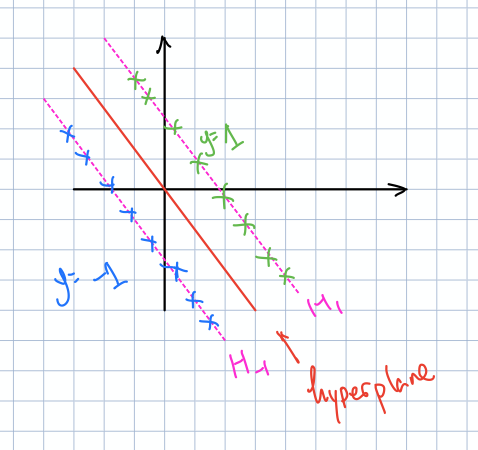
\includegraphics[height=190px]{Fig/q3-2}
	\end{note}
	
	\begin{note}[Parameter vector solution]{pink}{}
		2 points needed.
%		Write the parameter vector solution to the SVM problem as a linear combination of some points in your dataset.
%How many points did you require?
%[You may find built-in functions useful for this purpose.]
		
		$y = -0.5 x_{1999} + 0.5 x_{1998}$
	\end{note}
	
	\begin{note}[Mystery Dataset B]{pink}{}
		We ran into problem (infinity loop) with Hard-margin SVM, while Soft-margin SVM and Logistic regression has been successfully fitted. This is caused by the dataset that is inseparable with hard-margin, hence the program ran into infinity loop trying to separate the dataset that is not separable.

		192 points needed.
		
		
		To compare the SVM and logistic regression performance, the empirical metric accuracy is calculated based on test data: $\text{accuracy} = \frac{\text{\# right predictions}}{\text{\# of test data}}$
		
		We find:
		
		Soft-SVM Test Performance (Empirical Accuracy): 97.15\%
		
		Logit Test Performance (Empirical Accuracy): 96.95\%
		
		Hence, the Soft-SVM has better performance.
				
%Compute the solution for the same three methods on Mystery Dataset B. 
%You will again run into issues with one of them -- explain why. [The answer is likely to be simpler than last time.]

%Find a way to write the parameter vector solution to the SVM problem as a linear combination of some points in your dataset -- do not report the solution itself, but report how many points you used, and how you arrived at this answer.
%Compare the empirical prediction accuracy (i.e., using 0-1 loss) of the successfully-trained classifiers on the test set. 	

	\end{note}
\end{answer}


%%%%%%%%%%%%%%%
%%%% Ex 4 %%%%%
%%%%%%%%%%%%%%%
\newpage
\setcounter{section}{4}
\begin{exercise}[Support Vector Regression (8 pts)]{}
Let us consider support vector regression:
\begin{align}
\label{eq:CSVM}
\min_{\wv\in \RR^d, 
b\in\RR}  ~ \frac{1}{2} \|\wv\|_2^2 + C\sum_{i=1}^n \max\{ | y_i -  (\wv^\top \xv_i + b)| -\varepsilon , 0 \},
\end{align}
where $\xv_i \in \RR^d$, $y_i \in \RR$, and $\|\wv\|_2 := \sqrt{\sum_{j=1}^d w_j^2}$ is the Euclidean norm.

\begin{enumerate}
	
\item (2 pts) Derive the Lagrangian dual of the support vector regression loss function \eqref{eq:CSVM}. Please include intermediate steps so that you can get partial credits.

\ans{\mref{ans:4:1}} 


\vskip1cm

In the following you will complete and implement the following gradient algorithm for solving support vector regression in \Cref{eq:CSVM}:

\begin{algo}[GD for SVR.]{alg:CSVM}
	\DontPrintSemicolon
	\KwIn{$X\in\RR^{n\times d}$, $\yv\in \RR^n$, $\wv=\zero_d$, $b=0$, $\mathsf{max\_pass} \in \mathds{N}$, step size $\eta$}
	
	\KwOut{$\wv, b$}
	
	\For{$t=1, 2, \ldots, \mathsf{max\_pass}$ }{
		
		\For{$i=1, 2, \ldots, n$}{
			
			choose step size $\eta$
			
			\If{$|y_i - (\inner{\xv_i}{\wv}+b)| \geq \varepsilon$}{
				$\wv \gets $ \tcp*{$\xv_i$ is the $i$-th row of $X$}
				
				$b \gets $
			}	
			
			$\wv \gets $ \tcp*{proximal step}
		}
	}
\end{algo}

Note that this differs a bit from what you've seen so far, in terms of gradient descent. Rather than taking steps based on the entire loss function, we instead take a step based on the unregularized loss, and then perform a projection step based on the regularizer.

\item (2 pts) Compute the gradient \wrt $\wv$ and $b$ for each second term in \Cref{eq:CSVM}.
Note that in places where the function is non-differentiable, you might have to compute a sub-gradient.
\begin{align}
C\sum_{i=1}^n \max\{ | y_i -  (\wv^\top \xv_i + b)| -\varepsilon , 0 \}
\end{align}
	
	
\ans{\mref{ans:4:2}} 

	
\item (1 pt) Find the closed-form solution of the following proximal step:
	\begin{align}
	\mathsf{P}^\eta(\wv) = \argmin_{\zv} ~ \frac{1}{2\eta} \|\zv - \wv\|_2^2 + \frac{1}{2} \|\zv\|_2^2
	\end{align}
	
	
\ans{\mref{ans:4:3}} 

	
\item (3 pts) Implement \Cref{alg:CSVM}. You should use Ex 1.3 to complete lines 5-6, and Ex 1.4 for line 7. 
Run it on Mystery Dataset C (this is Mystery Dataset A from Assignment 1, but reused), and report your training error, training loss, and test error. Use $C=1$ and $\varepsilon = 0.1$.

\ans{\mref{ans:4:4}} 

\end{enumerate}
\end{exercise}


% --- ANS 4 --- %
\clearpage
\setcounter{answer}{0}
\begin{answer}[Lagrangian Dual Derivation]{ans:4:1}
	Let's substitute the regulation (second) term with a complement slack variables ($\xi_i, \xi_i'$) as suggested in lecture to account the delta error outside the $\epsilon$ margin.
	\begin{align}
		\textbf{Condition:}\\
		y_i - \hat{y}_i & \leq \xi_i + \epsilon \\
		\hat{y}_i - y_i & \leq \xi_i' + \epsilon \\
		\text{where } &  \,\xi_i,\xi_i'>0 , \quad \hat{y}_i = \wv^T \xv_i + b
	\end{align}

	\begin{center}
		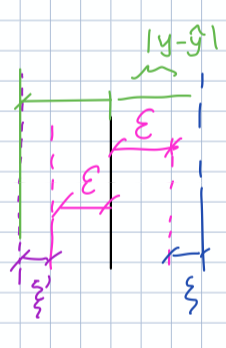
\includegraphics[height=150px]{Fig/slack}	
	\end{center}
		
	Hence, we may simplify the formulation \Cref{eq:CSVM} into:
	\begin{align}
			\min_{\wv\in \RR^d, 
b\in\RR}  ~ \frac{1}{2} \|\wv\|_2^2 + C\sum_{i=1}^n (\xi_i + \xi_i') & \\
		\textbf{where} &  \\
		y_i - \hat{y} & \leq \xi_i + \epsilon \\
		\hat{y} - y_i & \leq \xi_i' + \epsilon \\
		\text{where } &  \,\xi_i,\xi_i'>0 , \quad \hat{y} = \wv^T \xv_i + b
	\end{align}

	We may now apply Lagrangian with complement ($\alpha, \alpha'$) and ($\beta, \beta'$) multipliers:
	\begin{multline}
		\min_{w, b, \xi, \xi'} \quad \max_{\alpha, \alpha' \geq 0  \, \beta, \beta' \leq 0} 
		\frac12 \| \wv\|_2^2 + C\sum_{i=1}^n (\xi_i + \xi_i') 
		+ \sum_{i=1}^n \alpha_i (y_i - \hat{y}_i - \epsilon - \xi_i)  \\
		+ \sum_{i=1}^n \alpha_i' (- y_i + \hat{y}_i - \epsilon - \xi_i') 
		- \sum_{i=1}^n \beta_i \xi_i - \sum_{i=1}^n \beta_i' \xi_i' 
	\end{multline}	

	
	Swap min and max:
	\begin{multline}\label{eqn:lagrangian}
		\max_{\alpha, \alpha' \geq 0  \quad \beta, \beta' \leq 0} \quad \min_{w, b, \xi, \xi'} \frac12 \| \wv\|_2^2 + C\sum_{i=1}^n (\xi_i + \xi_i') 
		 + \sum_{i=1}^n \alpha_i (y_i -(\wv^T \xv_i + b) - \epsilon - \xi_i)  \\
		+ \sum_{i=1}^n \alpha_i' (- y_i + (\wv^T \xv_i + b) - \epsilon - \xi_i' ) 
		- \sum_{i=1}^n \beta_i \xi_i - \sum_{i=1}^n \beta_i' \xi_i' 
	\end{multline}
	
	Take derivative $\wrt w,b,\xi_i,\xi_i'$:
	\begin{align}
		\frac{\partial}{\partial \wv} &= \wv - \sum_{i=1}^n \alpha_i \xv_i + \sum_{i=1}^n \alpha_i' \xv_i\\
		\frac{\partial}{\partial b} &= - \sum_{i=1}^n \alpha_i + \sum_{i=1}^n \alpha_i'  \\
		\frac{\partial}{\partial \xi_i} & =nC - n\alpha_i - n\beta_i \\
		\frac{\partial}{\partial \xi_i'} & = nC - n\alpha_i' - n\beta_i' 
	\end{align}
	
	, and $\equiv 0$:
	\begin{align}
		\sum_{i=1}^n (\alpha_i  -  \alpha_i') \xv_i & = \wv \\
		\sum_{i=1}^n (\alpha_i' - \alpha_i) & = 0\\		
		\alpha_i + \beta_i = \alpha_i' + \beta_i' & = C
	\end{align}

	Substitute back to Lagrangian (\Cref{eqn:lagrangian}):
	\begin{multline}
		\max_{\alpha, \alpha' \geq 0  \quad \beta, \beta' \leq 0} \quad \frac12 \| \sum_{i=1}^n (\alpha_i  -  \alpha_i') \xv_i \|_2^2 + C\sum_{i=1}^n (\xi_i + \xi_i') 
		 + \sum_{i=1}^n \alpha_i (y_i -(\wv^T \xv_i + b) - \epsilon - \xi_i)  \\
		+ \sum_{i=1}^n \alpha_i' (- y_i + (\wv^T \xv_i + b) - \epsilon - \xi_i' ) 
		- \sum_{i=1}^n \beta_i \xi_i - \sum_{i=1}^n \beta_i' \xi_i' 
	\end{multline}
	\begin{multline}
		\max_{\alpha, \alpha' \geq 0  \quad \beta, \beta' \leq 0} \quad \frac12 \| \sum_{i=1}^n (\alpha_i  -  \alpha_i') \xv_i \|_2^2 + C\sum_{i=1}^n (\xi_i + \xi_i') 
		 + \sum_{i=1}^n \alpha_i y_i \cancel{- \sum_{i=1}^n \alpha_i (\wv^T \xv_i + b)} - \sum_{i=1}^n \alpha_i \epsilon -  \sum_{i=1}^n \alpha_i \xi_i  \\
		- \sum_{i=1}^n \alpha_i' y_i \bcancel{+ \sum_{i=1}^n \alpha_i' (\wv^T \xv_i + b)} - \sum_{i=1}^n \alpha_i' \epsilon -  \sum_{i=1}^n \alpha_i'\xi_i' 
		- \sum_{i=1}^n \beta_i \xi_i - \sum_{i=1}^n \beta_i' \xi_i' 
	\end{multline}
	\begin{multline}
		\max_{\alpha, \alpha' \geq 0  \quad \beta, \beta' \leq 0} \quad \frac12 \| \sum_{i=1}^n (\alpha_i  -  \alpha_i') \xv_i \|_2^2 + C\sum_{i=1}^n (\xi_i + \xi_i')
		  - \sum_{i=1}^n (\alpha_i+\alpha_i') \epsilon + \sum_{i=1}^n (\alpha_i'-\alpha_i)y_i\\ - 
		  \sum_{i=1}^n \cancelto{C}{(\alpha_i + \beta_i)} \xi_i
		-  \sum_{i=1}^n \cancelto{C}{(\alpha_i' + \beta_i')} \xi_i'
	\end{multline}
	\begin{equation}
		\max_{\alpha, \alpha' \geq 0} \quad \frac12 \| \sum_{i=1}^n (\alpha_i  -  \alpha_i') \xv_i \|_2^2 - \sum_{i=1}^n (\alpha_i+\alpha_i') \epsilon + \sum_{i=1}^n (\alpha_i'-\alpha_i)y_i
	\end{equation}
	
	Convert to minimization problem:
	\begin{note}[The Dual]{pink}{}
		\begin{equation}
			\min_{C \geq \alpha, \alpha' \geq 0} \quad \frac12 \sum_{i=1}^n \sum_{j=1}^n (\alpha_i  -  \alpha_i')(\alpha_j  -  \alpha_j') \xv_i^T \xv_j  + \epsilon \sum_{i=1}^n (\alpha_i+\alpha_i') - \sum_{i=1}^n (\alpha_i'-\alpha_i)y_i
		\end{equation}
		\begin{equation}
			\textbf{s.t.} \qquad \sum_{i=1}^n (\alpha_i' - \alpha_i) = 0
		\end{equation}
	\end{note}

\end{answer}

\newpage
\begin{answer}[Gradient]{ans:4:2}
	\begin{align}
		\frac{\partial}{\partial \wv} &= \sum_{i=1}^n
			\begin{cases}
				0 	  & |y_i - \hat{y}_i| \leq \epsilon \\
			 	- C x_i & y_i > \hat{y}_i , |y_i - \hat{y}_i| > \epsilon \\
				C x_i 	& \text{otherwise}
			\end{cases}		\\
		\frac{\partial}{\partial b} &= \sum_{i=1}^n
			\begin{cases}
				0 	& |y_i - \hat{y}_i| \leq \epsilon \\
				-C	& y_i > \hat{y}_i , |y_i - \hat{y}_i| > \epsilon \\
				C	& \text{otherwise}
			\end{cases}		\\
		& \text{where}\qquad \hat{y}_i = \wv^T \xv_i + b
	\end{align}
\end{answer}


\newpage
\begin{answer}[Closed Form Solution of the Proximal Step]{ans:4:3}
	\begin{align}
		\frac{\partial}{\partial z} \mathsf{P}^\eta(\wv) & = \frac{\partial}{\partial z} \left(\frac{1}{2\eta} \|\zv - \wv\|_2^2 + \frac{1}{2} \|\zv\|_2^2 \right)\\
		0 & = \frac{1}{\eta} (\zv - \wv) + \zv \\ 
		z & = \frac{w}{1+ \eta}
	\end{align}
	\begin{note}[Closed Form Solution]{pink}{}
		\begin{equation}
				z = \frac{w}{1+ \eta}	
		\end{equation}
	\end{note}
\end{answer}

\newpage
\begin{answer}[Implementation]{ans:4:4}
	\begin{algo}[Seudo implementation of GD for SVR.]{alg:CSVM:complete}
	\DontPrintSemicolon
	\KwIn{$X\in\RR^{n\times d}$, $\yv\in \RR^n$, $\wv=\zero_d$, $b=0$, $\mathsf{max\_pass} \in \mathds{N}$, step size $\eta$}
	
	\KwOut{$\wv, b$}
	
	\For{$t=1, 2, \ldots, \mathsf{max\_pass}$ }{
		
		\For{$i=1, 2, \ldots, n$}{
			
			choose step size $\eta$
			
			\If{$|y_i - (\inner{\xv_i}{\wv}+b)| \geq \varepsilon$}{
				$\wv \gets \wv - \eta C x_i \times \textbf{sgn}(<\wv, \xv> + b - y_i)$  \tcp*{$\xv_i$ is the $i$-th row of $X$}
				
				$b \gets  b - \eta C \times \textbf{sgn}(<\wv, \xv> + b - y_i)$
			}	
			
			$\wv \gets \frac{w}{1+\eta} $ \tcp*{proximal step}
		}
	}
	\end{algo}

	{
		\centering
		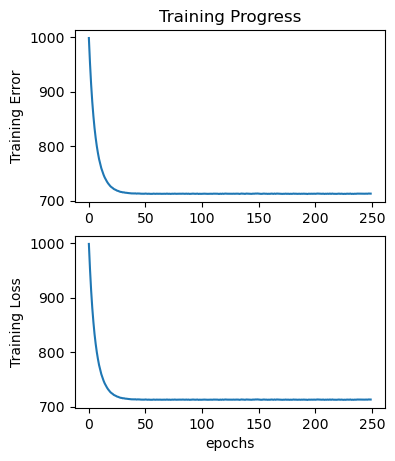
\includegraphics[height=300px]{../src_code/figs/ex4_training_progress_result.png}
		\captionof{figure}{Training Progress}
	}	
	
	\begin{lstlisting}[style=mystyle:output]
> [result  ] T: 249 | Training Error: 712.84065 | Training Loss: 713.37650 | Test Error: 891.05659
	\end{lstlisting}
\end{answer}

%%%%%%%%%%%%%%%%%%%%%%%%%%%%%%%%%%%%%%%%%%%%%%%%%%%%%%%%%%%%%%%%%%%%%%%%%%%%%%%%
%% ************************************************************************** %%
%% *                      TODO [Remove For Final Copy!]                     * %%
%% ************************************************************************** %%
%%%%%%%%%%%%%%%%%%%%%%%%%%%%%%%%%%%%%%%%%%%%%%%%%%%%%%%%%%%%%%%%%%%%%%%%%%%%%%%%
%\printlistoftodos

%%%%%%%%%%%%%%%%%%%%%%%%%%%%%%%%%%%%%%%%%%%%%%%%%%%%%%%%%%%%%%%%%%%%%%%%%%%%%%%%
%% ************************************************************************** %%
%% *                                Glossary                                * %%
%% ************************************************************************** %%
%%%%%%%%%%%%%%%%%%%%%%%%%%%%%%%%%%%%%%%%%%%%%%%%%%%%%%%%%%%%%%%%%%%%%%%%%%%%%%%%
% \clearpage
\printglossaries

%%%%%%%%%%%%%%%%%%%%%%%%%%%%%%%%%%%%%%%%%%%%%%%%%%%%%%%%%%%%%%%%%%%%%%%%%%%%%%%%
%% ************************************************************************** %%
%% *                               References                               * %%
%% ************************************************************************** %%
%%%%%%%%%%%%%%%%%%%%%%%%%%%%%%%%%%%%%%%%%%%%%%%%%%%%%%%%%%%%%%%%%%%%%%%%%%%%%%%%

% \printbibliography[heading=none]

%%%%%%%%%%%%%%%%%%%%%%%%%%%%%%%%%%%%%%%%%%%%%%%%%%%%%%%%%%%%%%%%%%%%%%%%%%%%%%%%
%% ************************************************************************** %%
%% *                               Appendices                               * %%
%% ************************************************************************** %%
%%%%%%%%%%%%%%%%%%%%%%%%%%%%%%%%%%%%%%%%%%%%%%%%%%%%%%%%%%%%%%%%%%%%%%%%%%%%%%%%
% appendices use section and subsection numbering
\clearpage
\appendix
\begin{appendices}
% INPUT UR APPENDIX
\end{appendices}

\end{document}


